
\documentclass{article}

\usepackage{amsmath}
\usepackage{amssymb}
\usepackage{amsthm}
\usepackage{natbib}
\usepackage{graphicx}
\usepackage{color}

% For algorithms
\usepackage[algoruled,vlined]{algorithm2e}
%\usepackage{algorithm}
\usepackage{algorithmic}

% Packages hyperref and algorithmic misbehave sometimes.  We can fix
% this with the following command.
% \newcommand{\theHalgorithm}{\arabic{algorithm}}



\SetKwInput{Input}{Input}

\newcommand{\union}{\cup}
\newcommand{\inter}{\cap}

\newcommand{\red}[1]{\textcolor{red}{#1}}

\begin{document}

\section{More candidate algorithms for OCC}
All of the algorithms here are similar to the clustering algorithms in that they are subset selection algorithms. (In clustering, we select a set of centers.) In the settings here, we are given a ground set $V$ of elements, and we are trying to select a subset to optimize an objective function $F: 2^V \to \mathbb{R}$.

\subsection{Greedy algorithms}
Many problems, such as maximizing a monotone increasing submodular function, e.g. to solve set cover, find a maximum spanning tree etc.\ are best solved using greedy algorithms.
In a serial setting, the algorithm proceeds as follows.
%\begin{figure}
%  \centering
  \begin{algorithm}
    \DontPrintSemicolon
    \caption{Greedy algorithm}
    \label{alg:greedy}
    \Input{set $V$, function $F$, budget constraint $k$} $S =
    \emptyset$\; \While{$S$ has not yet reached budget limits}
    { $i^* =
      \arg\max_{i \in V} F(S \union i)$\; 
      \If{$S \union i^*$ is within budget}{
        $S \leftarrow S \union i^*$\;}
      $V \leftarrow V \setminus i^*$\; } 
    return $S$\;
  \end{algorithm}
  
%  \caption{stuff}
%\label{fig:algo}
%\end{figure}


This algorithm solves two problems:
\begin{align}
  \max F(S) & \;\;\text{s.t. } |S| \leq k\\
  \min |S| & \;\;\text{s.t. } F(S) \geq \alpha.
\end{align}
The only change is the stoping criterion in the while loop that ensures we satisfy the constraint.

In a distributed setting, the data (points) would be distributed across workers, and in each epoch each worker would send its $b$ best candidates to the master, conditioned on the current global set $S$. 
This setup poses a few questions to address:
\begin{enumerate}\setlength{\itemsep}{0pt}
\item Can each worker locally compute or at least estimate $F(S \union i)$?
\item The above algorithm achieves an approximation factor of $1-1/e$ for Problem (1) and $O(\log n)$ for Problem (2). These factors only hold if the elements are added in the strictly greedy order (always the best). However, slightly looser bounds can be proved if we add an $i$ that satisfies $F(S \union i) \geq \beta F(S \union i^*)$. If each worker can compute $F$ accurately, then $i^*$ will be among the proposed points to add. How many more can we add without rejection and still maintain the $\beta$-factor?
\end{enumerate}
These questions are still substantial food for thought -- a relevant paper in this direction is \cite{chen13}. Other relevant papers are \citep{gomes10,golovin10}.

Alternatively, one can learn a policy that imitates the greedy algorithm (e.g. \cite{ross13} and references therein), and that can potentially be distributed too. Maybe it is  possible to have each worker learn a policy for its local data? Or each worker could run the policy locally on its own dat aset, and the master collects in the end.

\paragraph{Update.} A very recent parallel fast greedy method \cite{kumar13} could work in OCC too. It is based on filtering. The principle is like this: subsample a set of elements, and run the greedy algorithm on that. For all remaining elements, decide on an element-wise basis in parallel whether this would be a good addition to the set (formally, whether a greedy algorithm would include it in the set, possibly by throwing out an previously chosen element). This later step could be OCC-ified, if the assumption is that in the parallel step, not many additional elements are chosen. OCC could (hopefully) reduce the number of subsequent iterations, at the expense of some concurrency control.

As an explanantion, one could also run th egreedy algorithm as follows: pick the first $k$ elements, and then, when a new element arrives, swap it with a previously chosen element (if that increases the objective) or discard it. (This version gives a somewhat worse approximation factor of 1/2, however.)
One view on Kumar et al's algorithm is that the rounds of the filtering algorithm are ``corrections''. We first greedily pick something. Then, the set $M_S$ of all possible augmentations is determined in parallel. These are candidate augmentations but there is a lot of redundancy within the set $M_S$.
% \subsubsection{Online welfare maximization}


\subsection{Submodular maximization}
There is a recent, optimal and quite simple algorithm for maximizing arbitrary submodular functions \citep{buchbinder12}. In machine learning, such problems arise if we have e.g. summarization problems with a budget/cost penalty \citep{krause08}, MAP inference with determinantal point processes \citep{gillenwater12} or as subroutines in \citep{reed13}. Importantly, this algorithm could be an alternative if we replace the greedy problem above by $F(A) - \lambda |A|$.

The algorithm maintains two sets $A \subseteq B$, $A$ grows and $B$ shrinks. Initially, $A = \emptyset$ and $B = V$.
In each step, the algorithm looks at an uninspected point (in $B \setminus A$) and decides whether to keep it (add it to $A$) or discard it (remove it from $B$), based on the marginal gain of adding or discarding it. In the end, at termination, $A = B$. At any point in the algorithm, the points in $B$ are the accepted and the as yet uninspected points. (See also Figure~\ref{fig:serial_array}.)

The algorithm has two variants, a deterministic one with approximation factor $1/3$, and a randomized one with (expected) optimal approximation factor $1/2$. Algorithms~\ref{alg:usm_det} and \ref{alg:usm_rand} are both sequential algorithms.

\begin{figure}
  \centering
  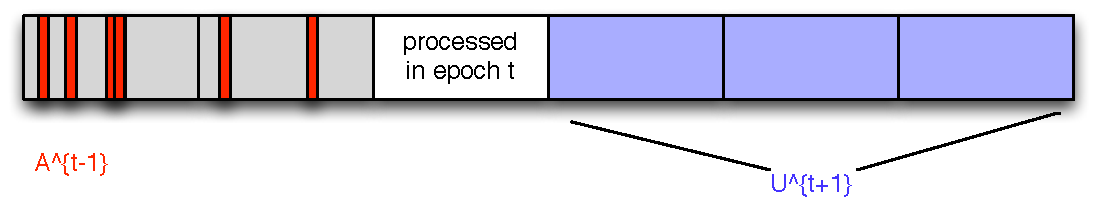
\includegraphics[width=0.85\textwidth]{serial_usmax}
  \caption{Illustration of sets for the serial algorithm. For both parallel and serial, we order points by epoch, and within each epoch by worker. The points processed in epoch $t$ are the points in $C_{j,t}$ for all $j$. When any point $i$ in the chunk of epoch $t$ is visited, $A$ contains $A^{t-1}$ (the red, selected points from previous epochs) in addition to any point selected in epoch $t$ before $i$; the set $B$ at that time contains $A$ and any unvisited point (i.e., $U^{t+1}$ and any unvisited point from epoch $t$).}
  \label{fig:serial_array}
\end{figure}

\begin{algorithm}
  \DontPrintSemicolon
  \caption{Deterministic submodular maximization}
  \label{alg:usm_det}
  $A = \emptyset$, $B = V$\;
  \For{$i=1$ to $n$}{
    $\Delta_{\text{add}}(i) = F(A \union i) - F(A)$\;
    $\Delta_{\text{rem}}(i) = F(B \setminus i) - F(B)$\;
    \If{$\Delta_{\text{add}}(i) \geq \Delta_{\text{rem}}(i)$}{
      $A \leftarrow A \union i$\;
    }
    \lElse{
      $B \leftarrow B \setminus i$\;
    }
  } 
  return $A$\;
\end{algorithm}

\begin{algorithm}
  \DontPrintSemicolon
  \caption{Randomized submodular maximization}
  \label{alg:usm_rand}
  $A = \emptyset$, $B = V$\;
  \For{$i=1$ to $n$}{
    $\Delta_{\text{add}}(i) = [F(A \union i) - F(A)]_+$\;
    $\Delta_{\text{rem}}(i) = [F(B \setminus i) - F(B)]_+$\;
    \If{with probability $\frac{\Delta_{\text{add}}(i)}{\Delta_{\text{add}}(i) + \Delta_{\text{rem}}(i)}$}{
      $A \leftarrow A \union i$\;
    }
    \lElse{
      $B \leftarrow B \setminus i$\;
    }
  } 
  return $A$\;
\end{algorithm}



In a distributed setting, the points are distributed across workers; worker $j$ owns chunk $C_j$. In epoch $t$, worker $j$ processes set $C_{j,t}$. Let $U^{t+1}$ denote all points that are processed after epoch $t$, i.e., $C_{j,t'}$ for $t' \geq t+1$ and all $j$.

The master maintains the global set $A^{t-1}$ in each epoch $t$ which contains the points of epochs $<t$ that have been accepted. Here, we assume that the optimal set $S^*$ is small compared to $V$. Here, we also assume that each worker can compute $F(S)$ on any $S \subseteq V$ (to be relaxed later).

In each epoch, worker $j$ selects candidate points from $C_{j,t}$ to be added to $A$. All other points from $C_{j,t}$ will count as discarded. At the end of the epoch, the master collects the proposed points and validates them, i.e., selects a final subset $S^t$ of those that will be added: $A^t = A^{t-1} \union S^t$. The points rejected by the master are also discarded. 
% The validated points are added to $A$.

If we do not want to miss any point in $S$, i.e., we want to be sure that any point a serial algorithm would select ends up being a candidate point, then we must locally overestimate $\Delta_{\text{add}}(i)$ and underestimate $\Delta_{\text{rem}}(i)$. 

Assume that in epoch $t$, the master visits the candidate points sequentially and grows $S^t$. At any such point, the sequential version of the algorithm would use $\Delta_{\text{add}}(i) =  F(A^{t-1} \union S^t \union i) - F(A^{t-1} \union S^t)$.
By submodularity,
\begin{align}
  \nonumber
  \Delta_{\text{add}}(i)\; :=\; &F(A^{t-1} \union S^t \union i) - F(A^{t-1} \union S^t)\; \leq\\
  &\qquad\qquad\qquad F(A^{t-1} \union i) - F(A^{t-1})\; =:\; \Delta_{\text{add}}^{t-1}(i).
\end{align}
Hence, it would be fine to locally use $\Delta^{t-1}_{\text{add}}(i)$ in epoch $t$.

Now let us look at $\Delta_{\text{rem}}(i)$.
After epoch $t$ is finished, the set $B$ consists of the accepted points $A^t$ of the points visited so far, and the unvisited points $U^{t+1}$, i.e., $B^t = A^t \union U^{t+1}$. When the serial algorithm processes $i \in C_{j,t}$ (for any $j$), it will compute $\Delta_{\text{rem}}(i)$ with respect to a set $B'$ that contains $A^{t-1} \union U^{t+1}$ and some more points from $U^t \setminus U^{t+1}$ (i.e., from the points visited in epoch $t$). Knowing this, we can again use submodularity to underestimate the serial $\Delta_{\text{rem}}(i)$:
%
%Furthermore, in epoch $t$, $B^t$ contains $A^{t-1} \union C_{1,t} \union C_{1,t+1} \union \ldots \union C_{2,t} \union C_{2,t+1} \union \ldots$. 
%for $\Delta^{t-1}_{\text{rem}}(i)$ it holds that 
\begin{align}
  \label{eq:1}
  \nonumber
  \Delta_{\text{rem}}(i) := &-\big(F(B') - F(B'\setminus i)\big) \geq\\
  &\qquad\qquad -\big(F(A^{t-1}\union U^{t+1}) - F(A^{t-1} \union U^{t+1} \setminus i)\big) =: \Delta^{t}_{\text{rem}}(i).
\end{align}
Algorithms~\ref{alg:worker} and \ref{alg:master} show the resulting algorithm. Since $\Delta_{\text{add}}^{t-1}(i) \geq \Delta_{\text{add}}(i)$ and $\Delta_{\text{rem}}^{t}(i) \geq \Delta_{\text{rem}}(i)$, the probabilities in the randomized algorithm are always in $[0,1]$.

\begin{algorithm}
  \DontPrintSemicolon
  \caption{Worker $j$ in epoch $t$}
  \label{alg:worker}
  $T_j = \emptyset$\;
  receive updated $A^{t-1}$\;
  \For{each point $i$ in $C_{j,t}$}{
    compute $\Delta_{\text{add}}^{t-1}(i)$ and $\Delta_{\text{rem}}^{t}(i)$\;
    deterministic: if $\Delta_{\text{add}}^{t-1}(i) \geq \Delta_{\text{rem}}^{t}(i)$ then $T_j = T_j \union i$\;
    randomized: with probability $\frac{\Delta_{\text{add}}^{t-1}(i)}{\Delta_{\text{add}}^{t-1}(i) + \Delta_{\text{rem}}^{t}(i)}$ do $T_j = T_j \union i$\;
  }
  send $T_j$ to master for validation\;
\end{algorithm}

\begin{algorithm}
  \DontPrintSemicolon
  \caption{Master in epoch $t$}
  \label{alg:master}
  collect proposals $T = \bigcup_j T_j$\;
  $S^t = \emptyset$\;
  \For{$i$ in $T$ in sequence}{
    compute $\Delta_{\text{add}}(i)$ and $\Delta_{\text{rem}}(i)$\;
    deterministic: if $\Delta_{\text{add}}(i) \geq \Delta_{\text{rem}}(i)$ then $T_j = T_j \union i$\;
    randomized: with probability $\frac{\Delta_{\text{add}}^{t-1}(i) + \Delta_{\text{rem}}^{t}(i)}{\Delta_{\text{add}}^{t-1}(i)}\cdot \frac{\Delta_{\text{add}}(i)}{\Delta_{\text{add}}(i) + \Delta_{\text{rem}}(i)}$ set $T_j = T_j \union i$\;
  }
\end{algorithm}

What is not shown is that we also need to keep track of $B$ (possibly indirectly). One option is that the local estimate of $\Delta_{\text{rem}}(i)$ is only computed from the local part of $U^{t+1}$, so that only $A^t$ is communicated. The master however needs to be able to compute the exact quantity. Or maybe there is a better idea\ldots Some functions may also admit to compute that more easily.


\paragraph{Where will this work?} Anything where $A$ and $B$ or conditional increment/decrement can be sketched, so that we do not need to communicate full sets and keep them around.
\begin{itemize}
\item Some of the algorithms by \citet{linB12learning} used for document summarization.
  Here are some candidates --- they can also be combined in arbiotrary ways:
  \begin{enumerate}
  \item We split the ground set into (possibly overlapping) groups $S_1, \ldots S_k$. The submodular function is
    \begin{equation}
      \label{eq:2}
      F(A) = \sum_{\ell=1}^k g\left(\sum_{i \in A \inter S_\ell} w_\ell(i)\right) - \lambda \sum_{i \in A}v(i),
    \end{equation}
    where $g$ is a nonnegative, nondecreasing scalar function and $w(i)$ and $v(i)$ ar nonnegative scalar weights.
    To evaluate this function, all that is needed is the group membership of the elements. Instead of the full sets $A$ and $B$, it is enough to maintain the sums $\sum_{i \in A \inter S_\ell} w(i)$, $\sum_{i \in B \inter S_\ell} w(i)$ and $\sum_{i \in V \inter S_\ell} w(i)$ to be able to compute the $\Delta$ values.
  The ``diversity shell components'' and the ROUGE-like loss in \citep{linB12learning} are of this form.
\item A special case is the set cover function (if the universe $U$ is not too large), where
  each element $i \in V$ indexes a set $C_i \subseteq U$ and we have the function
  \begin{equation}
    F(A) = |\bigcup_{i \in A}C_i|.
  \end{equation}
  In that case, each element $u \in U$ defines a group, and $w_u(i) = 1$ if $u \in C_i$, and $w_u(i) = 0$ otherwise. The concave function $g$ in that case is $g(y) = \min\{1,y\}$.
\item We again split the ground set into groups, but this time, instead of $g(\sum_{i \in A \inter S_\ell} w(i))$, use
   \begin{equation}
      \label{eq:3}
      F(A) = \sum_{\ell=1}^k (\max_{i \in A \inter S_\ell} w(i)) - \lambda \sum_{i \in A}v(i),
    \end{equation}
    The ``clustered facility location shell components'' in \citep{linB12learning} are of this form.   Here, the sketches contain the maximum elements of each group.
  \end{enumerate}
  Similar functions are also used in \citep{linB11,liu13}.
 \item Probabilistic coverage \citep{yue11}. These are functions of the form
    \begin{equation}
      \label{eq:4}
      F_i(A) = 1 - \prod_{a \in A}(1-P(i\mid a)).
    \end{equation}
    In the application in \citep{yue11}, $P(i \mid a)$ is the probability that topic $i$ is covered by article $a$. We here have one function $F_i$ per topic $i$ and need to maintain the products $\prod_{a \in A}(1-P(i\mid a))$ as a sketch for $A$.
\item quadratic functions like max-cut? (symmetric functions?)
\end{itemize}


\section{Document Summarization}

We base our survey on \citep{linB12learning}. 

\paragraph{Data} They use the NIST DUC 2003--2007 data. \red{Size of data?}

DUC-03 has 60 document clusters.


\paragraph{Tasks} They show 2 tasks: (1) query-independent summarization (DUC-03, DUC-04) and (2) query-focused summarization (DUC-05, DUC-06, DUC-07). 


\paragraph{Submodular functions}
\begin{description}
\item[diversity components]
  \begin{equation}
    \label{eq:6}
    F^{\text{div}}(S) = \frac{\sum_{k=1}^K(\sum_{i \in S \inter P_k}r_i)^a}{\zeta},
  \end{equation}
  with a constant $\zeta = \sum_{k=1}^K(\sum_{i \in P_k}r_i)^a$ that can be easily precomputed in a distributed fashion if the $r_i$ and clusters $P_k$ are known. Such functions favor to choose elements from different clusters.
  This function needs \emph{a clustering, definition of $a$, singleton rewards $r_i \in [0,1]$}. This function can be sketched by keeping the sums of $r_i$ for each cluster.
\item[FL components]
  \begin{equation}
    \label{eq:7}
    F^{\text{FL}}(S) = \frac{1}{K}\sum_{k=1}^K \max_{i \in S \inter P_k} r_i.
  \end{equation}
  Similar effect as the above, but even more extreme: only the max $r_i$ of each $P_k$ counts.
  This function needs \emph{a clustering, and  singleton rewards $r_i \in [0,1]$}.
  This function can be sketched by keeping the max of $r_i$ for each cluster.
\item[fidelity component]
  \begin{equation}
    \label{eq:8}
    F^{\text{fid}}(S) = \frac{1}{|V|} \sum_{i \in V} \min\{ \frac{\mathcal{C}_i(S)}{\zeta_2}, \alpha \},
  \end{equation}
  for a pre-computable constant $\zeta_2 = \mathcal{C}_i(V)$, and
  \begin{equation}
    \label{eq:5}
    \mathcal{C}_i(S) = \sum_{j \in S} s(i,j),
  \end{equation}
  where $s(i,j)$ is the similarity between elements $i$ and $j$. \emph{In the paper, they write that they sum over $j \in V$ -- summing over $j \in S$ makes more sense to me.} This function needs \emph{similarities, and a definition of $\alpha$.}
  Unfortunately, for the marginal gain $F(j | S)$ of this function, we need to know $\mathcal{C}_i(j)$ and $\mathcal{C}_i(S)$ for all elements $i \in V$, unless we have reached the saturation threshold already. \emph{Efficient approximations: (1) Can we use only similarities to the $M$ nearest neighbors, or the $\epsilon$-closest neighbors? (2) assume that the sentences have been randomly distributed across processors, and estimate the gain locally only; (3) use approximate matrix multiplication by sampling the similarity matrix.}
\end{description}

\paragraph{Submodular functions for (1)} For (1), they used the ROUGE-like loss ($\omega_e = 1$) and 15 variants of 
fidelity components, with 5 different $\alpha$'s, in $\{0.01, \ldots, 0.05\}$.

\paragraph{Submodular functions for (2)}
This uses diversity components, facility location components and fidelity components. They used 3 different clusterings ($K = 0.1|V|$, $K=0.2|V|$, $K=0.3|V|$).

6 clustered FL components (3 clusterings, 2 types of singleton rewards); 18 diversity components (3 clusterings, 2 types of singleton rewards, 3 curvatures $a=0.5, 0.6, 0.7$).


\paragraph{Submodular loss function for learning}
They use $1-\ell_{ROUGE}$ for
\begin{equation}
  \label{eq:9}
  \ell_{ROUGE}(S) = \zeta_3^{-1}\sum_{e \in \overline{R}}\omega_e c_e(S),
\end{equation}
where $N$ is the set of all $n$-grams, and $c_e$ the number of times $n$-gram $e$ occurs in summary $S \subseteq V$, i.e., $c_e(S) = \sum_{i \in S} \delta_{e,i}$, and $\delta_{e,i} = 1$ iff $i$ contains $e$. Here, we sum over $\overline{R} = N \setminus (\union_i R_i)$, where $R_i$ is the set of $n$-grams contained in reference summary $i$. The constant is $\zeta_3 = \sum_{e \in \overline{R}}\omega_e c_e(V)$.


\paragraph{Elements needed for implementation}
\begin{description}
\item[similarity function $s(i,j)$ between sentences] they use 3 variants:
  (a) cosine similarity with unigram TF-IDF vector; (b) cosine similarity with bigram TF-IDF vector; (c) cosine similarity with vector generated by LSI.
\item[clustering of sentences] They have 3 different numbers of clusters. \emph{Could implement that with DP-means with 3 different $\lambda$.}
\item[query-independent singleton rewards $r_i$] There is a singleton reward for each sentence: similarity of $i$ with all other sentences in $V$. \emph{needs to be computed once in the beginning --- can we smartly distribute that? I presume it is Eqn~\ref{eq:5} with $S=V$. ``Sketch'' needed from each processor: for each feature $k$, sum $x_{ik}/\|x_i\|$ and send sum. May be a lot if features are very high dimensional. Can we hash?}
\item[query-dependent singleton rewards $r_i$] number of terms (up to bi-grams) that sentence $j$ overlaps with query $Q$. \emph{easy to compute locally if query is known.}
  
\end{description}


\section{Social Networks}


\bibliographystyle{abbrvnat}
\bibliography{../../Dropbox/generic/allrefs}

\end{document}
